\section{Bausteinsicht}

\subsection{Ebene 1: Das Gesamtsystem}

Das System besteht aus sieben eigenständig ausgelieferten Bausteinen sowie
einem Nachrichtenbroker und einem Loadbalancer.
Die Aufteilung orientiert sich an den fachlichen Verantwortungsbereichen des Systems.
Abbildung~\ref{fig:bausteinsicht} zeigt den Aufbau des Systems.

\begin{figure}[H]
    \centering
    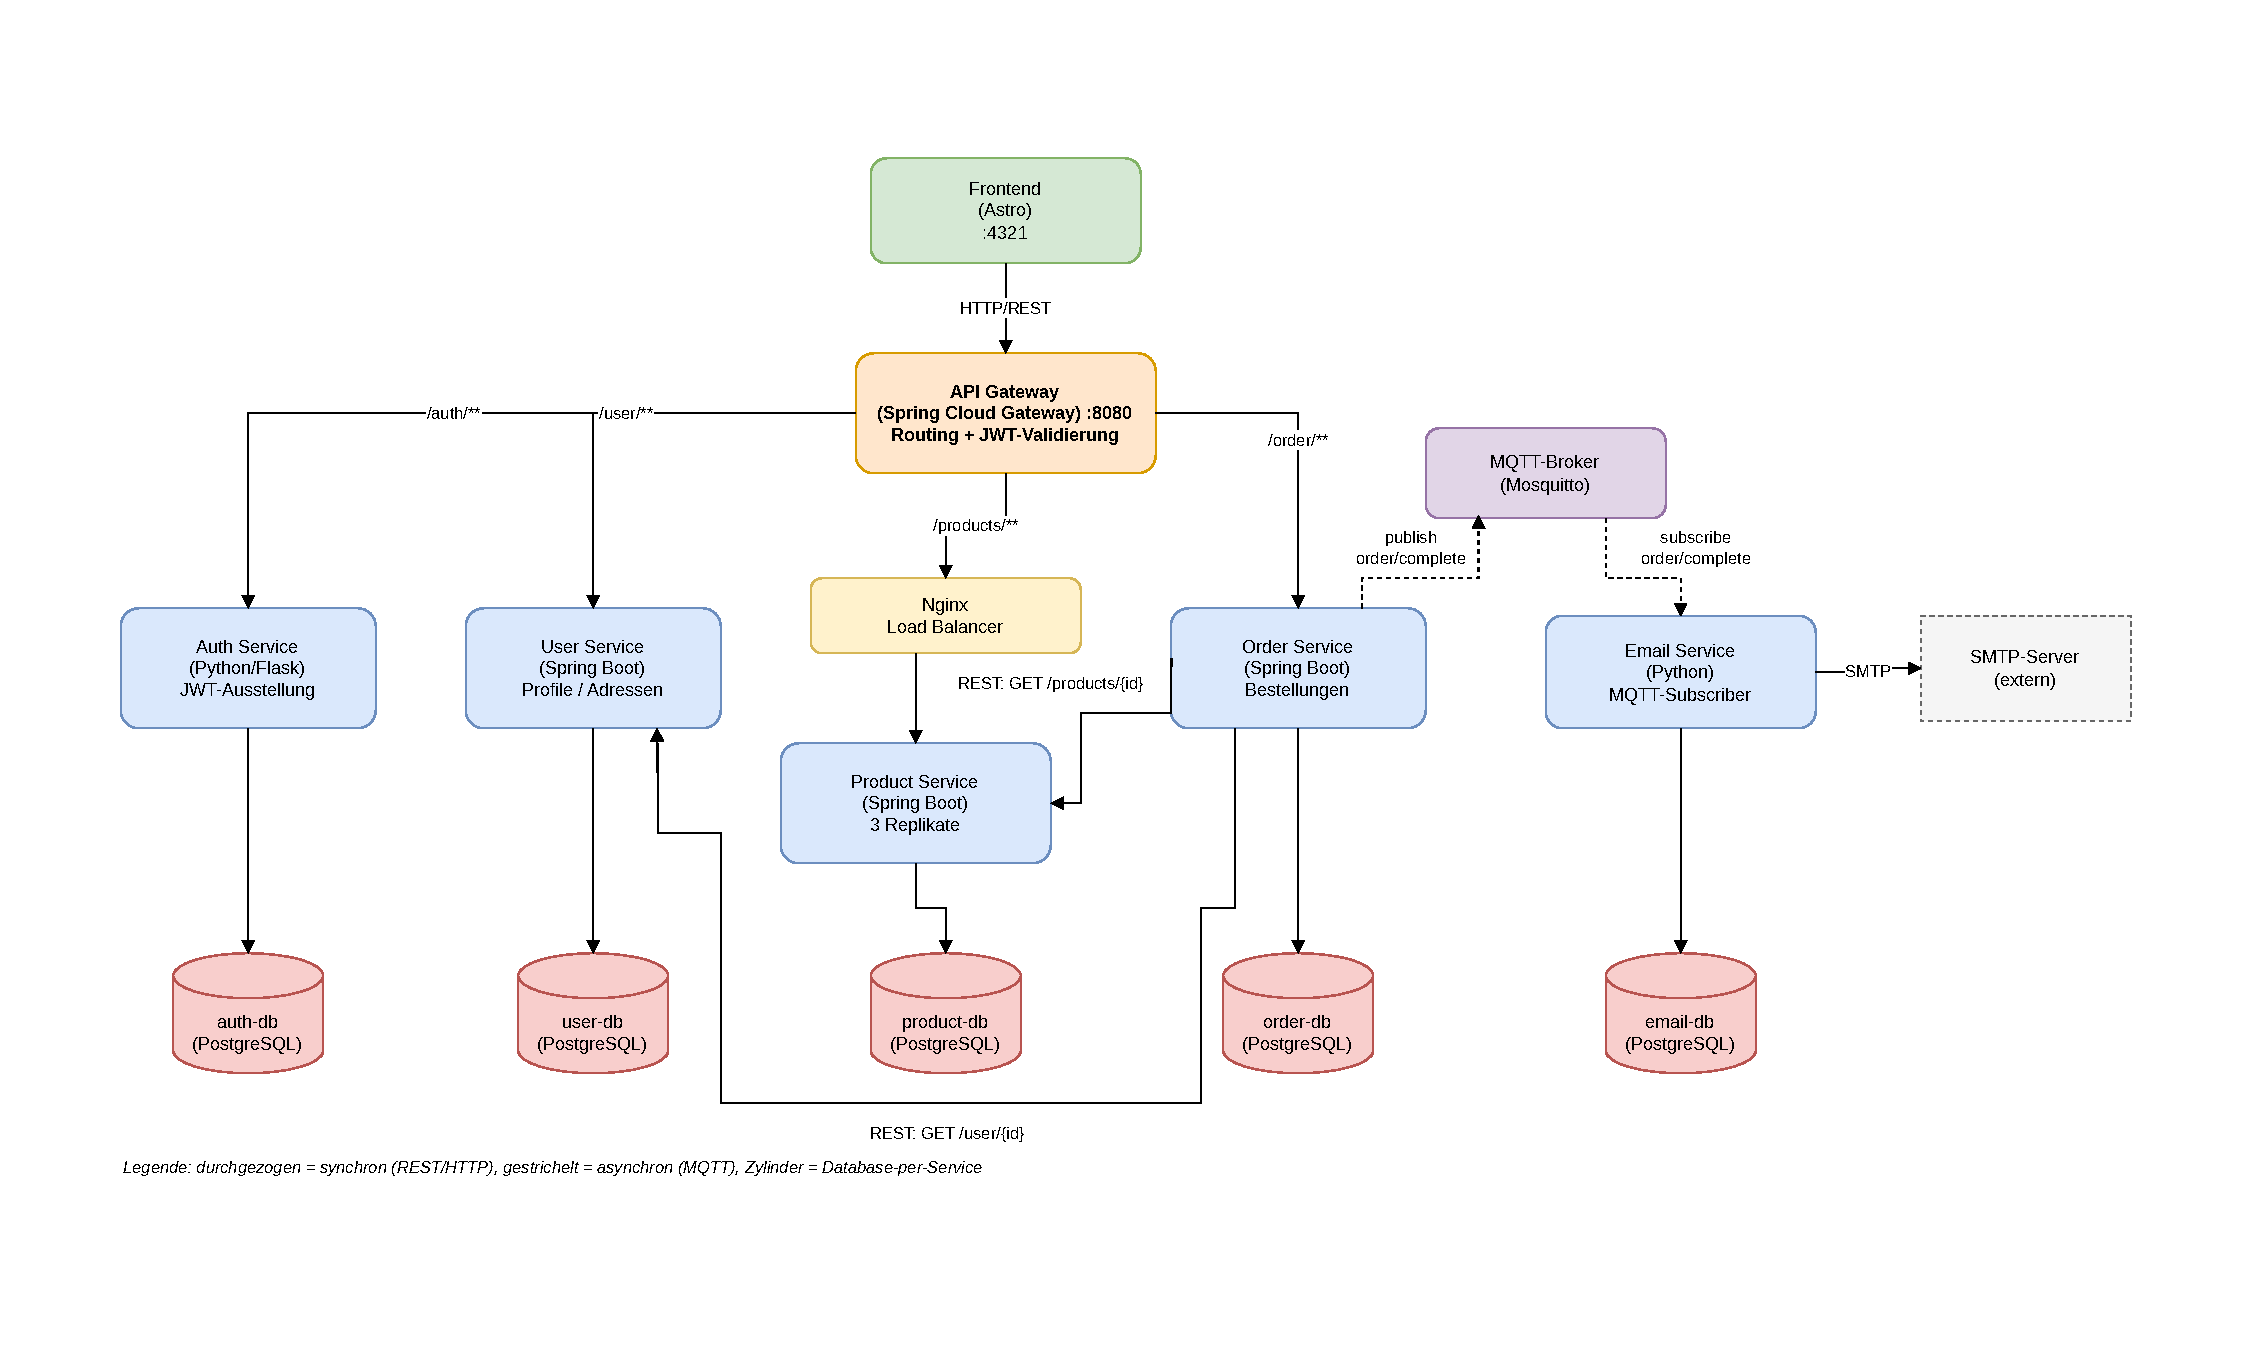
\includegraphics[width=\linewidth,trim=2cm 2cm 2cm 2cm,clip]{images/02-bausteinsicht}
    \caption{Bausteinsicht}
    \label{fig:bausteinsicht}
\end{figure}

Die Verantwortlichkeiten der einzelnen Bausteine sind in Tabelle~\ref{tab:bausteine} zusammengefasst.
    {
    \renewcommand{\arraystretch}{1.5}

    \begin{longtable}{@{}
            >{\bfseries\raggedright\arraybackslash}p{0.18\linewidth}
            >{\raggedright\arraybackslash}p{0.82\linewidth}
        @{}}
        \caption{Verantwortlichkeiten der Bausteine}
        \label{tab:bausteine} \\

        \toprule
        \rowcolor{tableHeaderColor}
        Baustein & Verantwortung \\
        \midrule
        \endfirsthead

        \multicolumn{2}{@{}l}{%
            \tablename\ \thetable{} -- Fortsetzung
        } \\

        \toprule
        \rowcolor{tableHeaderColor}
        Baustein & Verantwortung \\
        \midrule
        \endhead

        \midrule
        \multicolumn{2}{r@{}}{Fortsetzung auf der nächsten Seite} \\
        \endfoot

        \bottomrule
        \endlastfoot

        Frontend &
        Mit Astro und SolidJS umgesetzt. Stellt Komponenten und Seiten für
        Produkte, Warenkorb und Benutzerkonto bereit. \\

        \rowcolor{tableRowColor}
        API Gateway &
        Als Spring-Cloud-Gateway-Anwendung umgesetzt. Enthält die Routen zu den
        Services sowie einen Filter zur JWT-Validierung. \\

        Auth Service &
        Als Flask-Anwendung umgesetzt. Enthält REST-Endpunkte für Registrierung
        und Anmeldung sowie die Erzeugung von JWTs. \\

        \rowcolor{tableRowColor}
        User Service &
        Als Spring-Boot-Anwendung mit Controller-, Service- und
        Repository-Schicht umgesetzt. Verwaltet Benutzerprofile und
        Lieferadressen. \\

        Product Service &
        Als Spring-Boot-Anwendung mit Controller-, Service- und
        Repository-Schicht umgesetzt. Verwaltet Produkte und deren
        Verkaufsstatus. \\

        \rowcolor{tableRowColor}
        Order Service &
        Als Spring-Boot-Anwendung umgesetzt. Koordiniert den Kaufvorgang über
        REST-Clients, speichert Bestellungen und veröffentlicht
        Bestellereignisse über MQTT. \\

        Email Service &
        Als Python-Anwendung mit \texttt{paho-mqtt} umgesetzt. Abonniert
        Bestellereignisse, rendert E-Mail-Vorlagen und versendet
        Bestellbestätigungen. \\

        \rowcolor{tableRowColor}
        MQTT-Broker &
        Vermittelt die asynchronen Bestellereignisse zwischen Order Service
        und Email Service. \\

        Nginx &
        Verteilt Produktanfragen im Round-Robin-Verfahren auf die drei
        Instanzen des Product Service. \\

    \end{longtable}
}

\subsection{Ebene 2 -- Order Service (exemplarisch)}

Der Order Service ist intern in Controller, Geschäftslogik,
Datenzugriff und ausgehende Clients gegliedert.
Die ausgehenden REST- und MQTT-Aufrufe sind in eigenen Client-Klassen gekapselt.
Dadurch bleibt die eigentliche Kaufabwicklung im \texttt{OrderService} weitgehend unabhängig von den verwendeten Kommunikationsprotokollen.

Tabelle~\ref{tab:order-codebausteine} beschreibt die wichtigsten
Codebausteine und Abbildung~\ref{fig:order_service} zeigt deren
Abhängigkeiten.
\begin{table}[H]
    \centering
    \caption{Codebausteine des Order Service}
    \label{tab:order-codebausteine}

    \renewcommand{\arraystretch}{1.4}

    \begin{tabularx}{\linewidth}{@{}
            >{\bfseries\raggedright\arraybackslash}p{0.27\linewidth}
            >{\raggedright\arraybackslash}X
        @{}}

        \toprule
        \rowcolor{tableHeaderColor}
        Codebaustein & Aufgabe \\
        \midrule

        OrderController &
        Stellt die REST-Endpunkte des Order Service bereit, nimmt Anfragen
        entgegen und delegiert die Verarbeitung an den
        \texttt{OrderService}. \\

        \rowcolor{tableRowColor}
        OrderService &
        Enthält die Geschäftslogik des Kaufvorgangs. Prüft Produkte,
        reserviert Artikel, legt Bestellungen an und löst die
        Bestellbestätigung aus. \\

        OrderRepository &
        Kapselt mit Spring Data JPA den Zugriff auf die
        \texttt{order-service-db}. \\

        \rowcolor{tableRowColor}
        ProductServiceClient &
        Kapselt die REST-Aufrufe zum Product Service, beispielsweise zum
        Abrufen, Reservieren und Freigeben eines Produkts. \\

        UserServiceClient &
        Ruft die Benutzerdaten und die E-Mail-Adresse des Käufers beim
        User Service ab. \\

        \rowcolor{tableRowColor}
        EmailServiceClient &
        Veröffentlicht nach einem erfolgreichen Kauf ein MQTT-Ereignis auf
        dem Topic \texttt{order/complete}. \\

        OrderStatusScheduler &
        Sucht regelmäßig nach fälligen Bestellungen und führt die
        Statusübergänge \texttt{CREATED}, \texttt{PAID},
        \texttt{SHIPPED} und \texttt{DELIVERED} aus. \\

        \rowcolor{tableRowColor}
        GlobalExceptionHandler &
        Wandelt Exceptions in einheitliche HTTP-Fehlerantworten um. \\

        DTOs und Domänenklassen &
        Enthalten die internen Bestellobjekte sowie die Datenmodelle für die
        Kommunikation mit Product Service und User Service. \\

        \bottomrule
    \end{tabularx}
\end{table}

\begin{figure}[H]
    \centering
    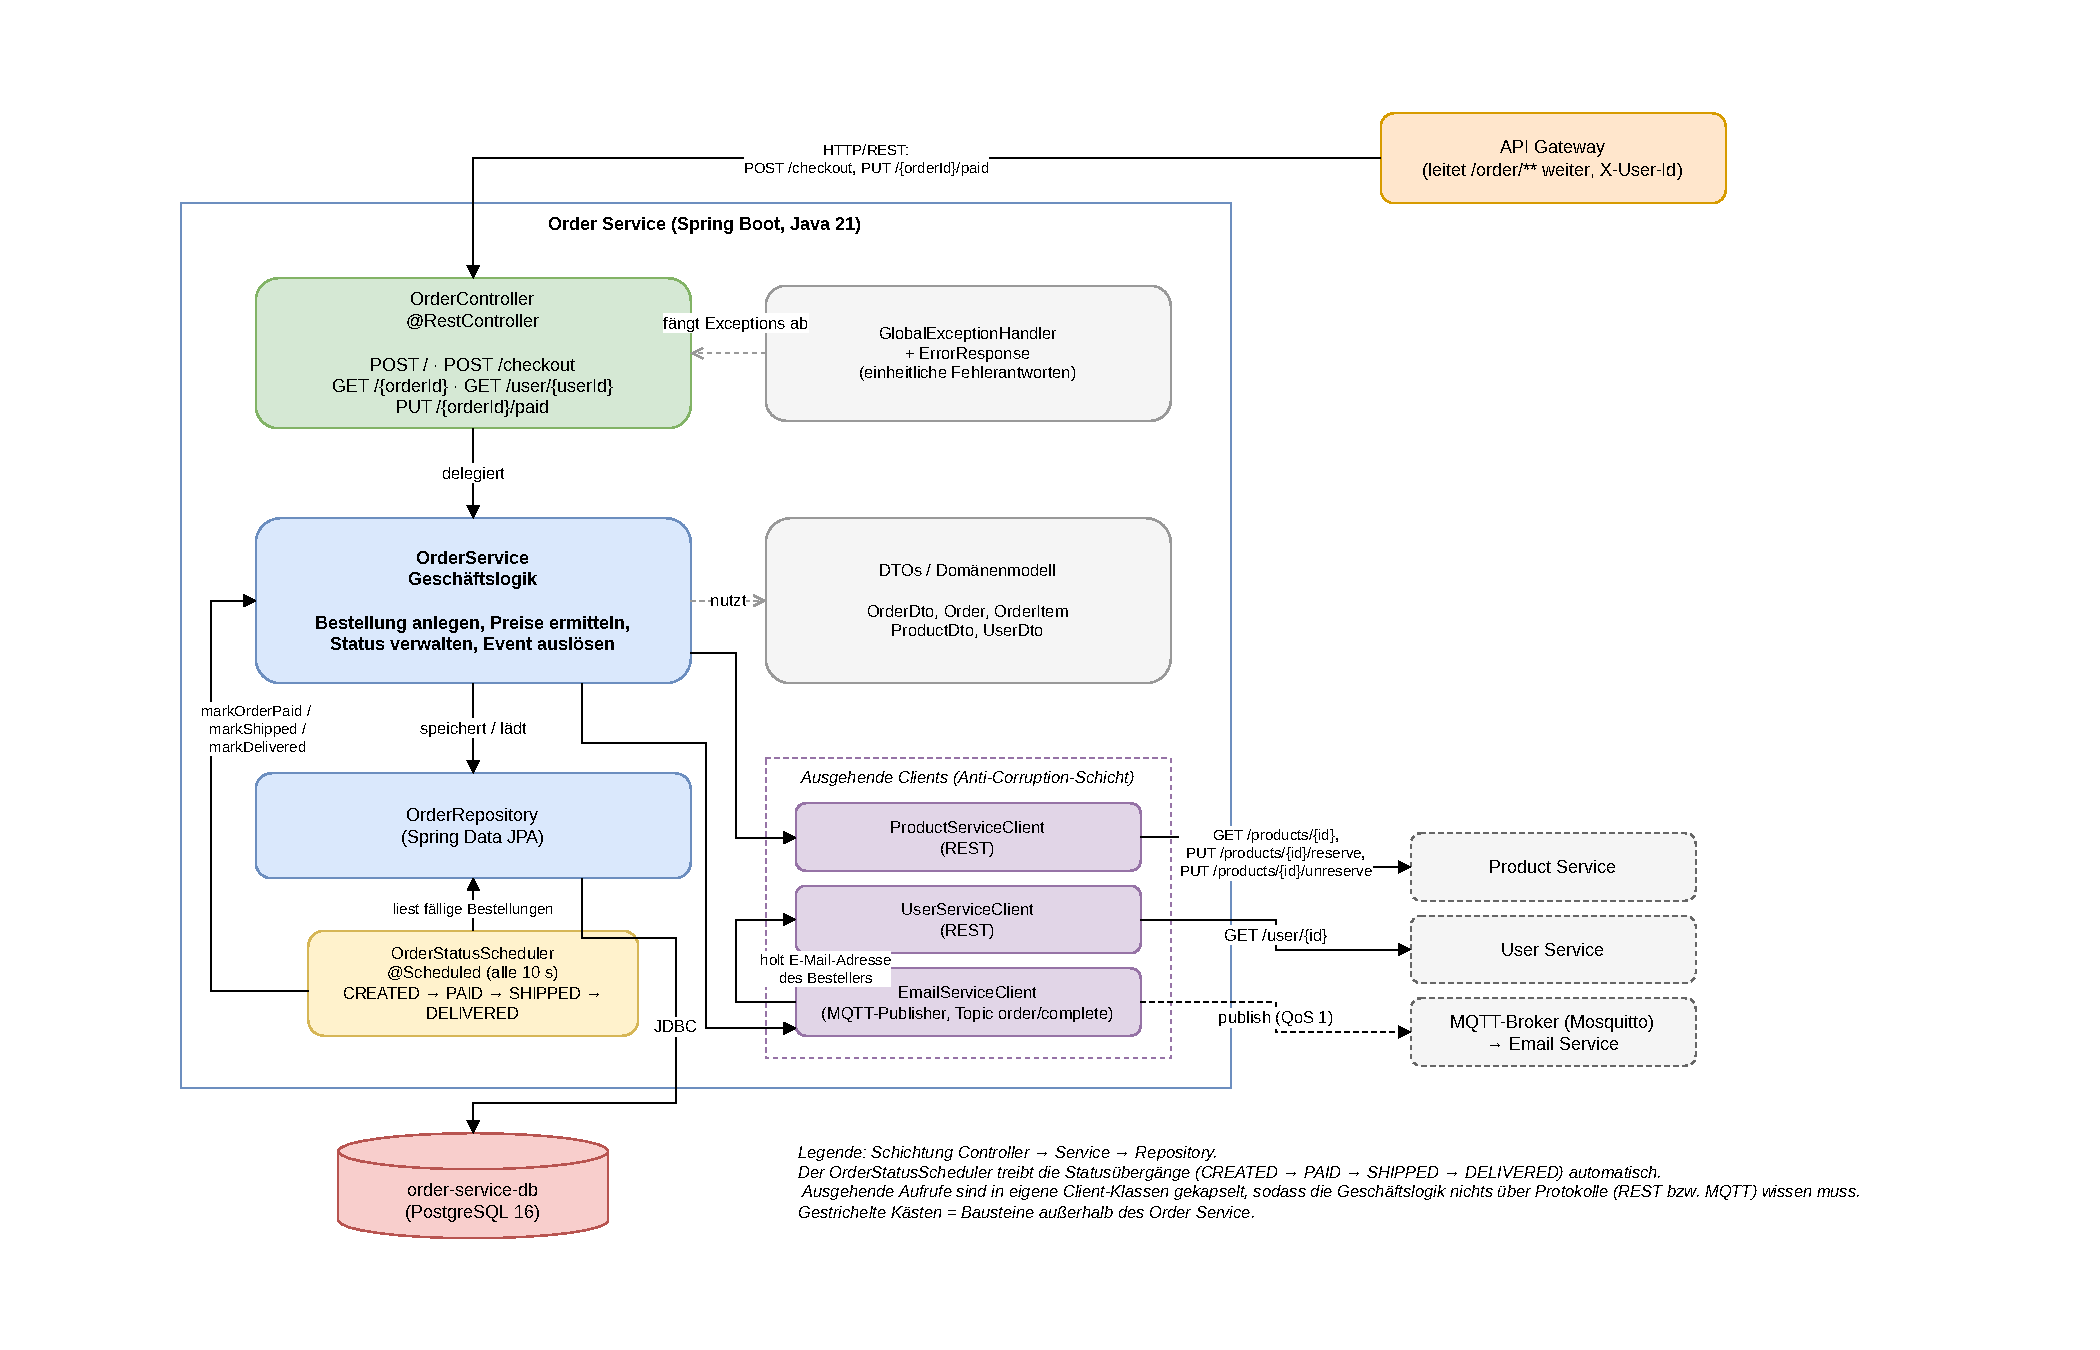
\includegraphics[width=\linewidth,trim=3cm 1cm 4cm 1cm,clip]{images/06-whitebox-order-service}
    \caption{Order Service}
    \label{fig:order_service}
\end{figure}
